\documentclass[15pt]{beamer}
%
% Choose how your presentation looks.
%
% For more themes, color themes and font themes, see:
% http://deic.uab.es/~iblanes/beamer_gallery/index_by_theme.html
%
\mode<presentation>

{
  \usetheme{PaloAlto}      % or try Darmstadt, Madrid, Warsaw, ...
  \usecolortheme{whale} % or try albatross, beaver, crane, ...
  \usefonttheme{default}  % or try serif, structurebold, ...
  \setbeamertemplate{navigation symbols}{}
  \setbeamertemplate{caption}[numbered]
} 
%remove navigation symbols at bottom
\setbeamertemplate{navigation symbols}{}
\setbeamertemplate{footline}[frame number]
\setbeamertemplate{footline}[text line] {

	\makebox[.7\paperwidth]{
		\insertframenumber  /\inserttotalframenumber
		\hfill
		\url{http://envirohack.herokuapp.com/}
	}

}

% add logo
\usepackage{pgf}
%coords are in relation to lower right corner
\logo{\pgfputat{\pgfxy(-1,8)}{\pgfbox[center,base]{
\includegraphics[width=1.7cm]{logo.jpg}}}}


%I had problems compiling doc on X230 without next two lines
\usepackage{etex}
\reserveinserts{28}
%On X530 it worked without problems

%\usepackage[utf8x]{inputenc}
%My std preamble for the docs
%\selectlanguage{british}%
\usepackage[british]{babel}
\usepackage{microtype} %better text
\IfFileExists{lmodern.sty}{\usepackage{lmodern}}{} %type 1 vector font
%
\usepackage{lettrine}
\usepackage{listings} %Add list support
\usepackage{colortbl} %colors in TABLES
%\usepackage{tikz,amsmath, amssymb,bm,color}
\usepackage{nicefrac}
\usepackage{lastpage} %get last page

%COLORS
\usepackage{color}
\definecolor{lightgray}{gray}{0.8} %for colortbl


%%%%%%%%%%%%%%%%%%%%%%%%%%%%%%%%%%%%%%%%%%%%%%%%%%%%%%%%%%%%%%%%%%
%FOOTNOTES
%nice look after http://www.dedoimedo.com
\usepackage[bottom,hang,splitrule]{footmisc} %\usepackage[bottom]{footmisc}
\setlength{\footnotemargin}{0.35cm} %space between number and footnote text
\setlength{\footnotesep}{0.2cm} %{12pt} %space between footnotes
\setlength{\skip\footins}{0.3cm} % space between the text body and the footnotes
%\setlength{\footskip}{0pt} dont do it. It will overflow page no

%%%%%%%%%%%%%%%%%%%%%%%%%%%%%%%%%%%%%%%%%%%%%%%%%%%%%%%%%%%%%%%%%%%
%TABLE SETTINGS
\usepackage{colortbl} %colors in table
\usepackage{rotating} %rotatins within tables
\usepackage{multirow}
\renewcommand{\arraystretch}{1.2} %add padding/spacing
%\usepackage{adjustbox}%rotating and fitting into page
%

\usepackage{booktabs} % To thicken table lines
%define thickness of table lines
\let\mytoprule\toprule
\renewcommand{\toprule}{\mytoprule[0.20em]}
\let\mytoprule\bottomrule
\renewcommand{\bottomrule}{\mytoprule[0.20em]}
\let\mytoprule\midrule
\renewcommand{\midrule}{\mytoprule[0.08em]}

\usepackage{spreadtab} % for simple calculations

%vertically and horizontally centered multicolumn cells with a fixed width. M{width}
%\newcolumntype{M}[1]{>{\centering\hspace{0pt}}m{#1}}
% each spanned cell has the same width. S{width of multicolumn cell}{number of spanned columns}
%\newcolumntype{S}[2]{>{\centering\hspace{0pt}}m{(#1+(2\tabcolsep+\arrayrulewidth)*(1-#2))/#2}}

%%%%%%%%%%%%%%%%%%%%%%%%%%%%%%%%%%%%%%%%%%%%%%%%%%%%%%%%%%%%%%%%%%%
%TikZ
\usepackage{tikz}

\colorlet{red}{red!50}
\colorlet{green}{green!50}
\colorlet{blue}{blue!50}
\definecolor{yellow}{HTML}{FFFF00}
\colorlet{yellow}{yellow!50}
\definecolor{fiolet}{HTML}{7030A0}
\colorlet{fiolet}{fiolet!50}
\colorlet{bgd_main}{black!50}
\colorlet{bgd}{bgd_main!75}
\colorlet{bgd2}{bgd_main!50}
\colorlet{bgd3}{bgd_main!25}
\colorlet{bgd4}{bgd_main!15}

\usetikzlibrary{shapes,arrows,calc,positioning}

%%%%%%%%%%%%%%%%%%%%%%%%%%%%%%%%%%%%%%%%%%%%%%%%%%%%%%%%%%%%%%%%%%%
% Footnotes in Figs
%\rule[raise-height]{width}{thickness}
\newcommand*{\FigFootnote}[1]{
\noindent \begin{flushleft}
\rule[0.2ex]{0.4\columnwidth}{0.5pt}
\par
\footnotesize
#1
\footnotesize
\end{flushleft}
}

%%%%%%%%%%%%%%%%%%%%%%%%%%%%%%%%%%%%%%%%%%%%%%%%%%%%%%%%%%%%%%%%%%%
%MATH, number display
%need to install siunitx, l3kernel,l3packages
\usepackage{siunitx} %this is for units display

\sisetup{per-mode=fraction, tight-spacing = true , fraction-function = \nicefrac, quotient-mode = fraction}% %nicefrac \tfrac
\sisetup{inter-unit-product = \ensuremath { { } \cdot { } } , exponent-product = \cdot }%
\sisetup{input-product=x , output-quotient =  \ensuremath { { } \times{}}} %for 1x2x3
%number grouping(3), std==true %\sisetup{group-digits = decimal} 
\sisetup{group-minimum-digits = 4} %start grouping from 4 digits, in 3 no groups
\sisetup{range-units = single,range-phrase = \,--\,} %2-3C not 2C-3C %, range-phrase = --
\sisetup{separate-uncertainty=true} %2+-1 not 2(1)
\sisetup{prefixes-as-symbols=true } % , scientific-notation = engineering false for 10^-9 ect ect , exp in multiple of 3
\sisetup{range-phrase = \,-\, } % , refo of ranges
%\sisetup{zero-decimal-to-integer, round-mode = places,round-precision = 3}
%\sisetup{add-arc-degree-zero=true , add-arc-minute-zero=true ,add-arc-second-zero=true} %for angle settings

%This is to auto convert ns,ms,us to 10^-xx s
\DeclareSIUnit[scientific-notation = engineering, prefixes-as-symbols=false]{\psec}{\pico\second}
\DeclareSIUnit[scientific-notation = engineering, prefixes-as-symbols=false]{\nsec}{\nano\second} 
\DeclareSIUnit[scientific-notation = engineering, prefixes-as-symbols=false]{\usec}{\micro\second}
\DeclareSIUnit[scientific-notation = engineering, prefixes-as-symbols=false]{\msec}{\milli\second} 

%...AND SOME UNITS
\DeclareSIUnit\dBm{dBm}
\DeclareSIUnit\ppm{ppm} %{\num{1e-6}}%{ppm}
\DeclareSIUnit\yr{yr} %{{361}\day}<-nice nice
\DeclareSIUnit\cy{cycle} %phase cycle
\DeclareSIUnit\epoch{epoch} %GPS/LL epoch
\DeclareSIUnit\inch{"} %inch 
\DeclareSIUnit\wk{week} %week
\DeclareSIUnit\hr{hrs} %hours
\DeclareSIUnit\min{minute} %hours
\DeclareSIUnit\mile{mi}
\DeclareSIUnit\Mcps{Mcps}
\DeclareSIUnit\bit{bit}
\DeclareSIUnit\chip{chip length}
%Other units
\newcommand*{\GBP}[1]{$\SI{#1}[\textsterling]{}$}


%%%%%SHORTHANDS (Standard Sentences)
%\newcommand*{\Myrange}[3]{$\textrm{\SIrange{#1}{#2}{#3}}$}

%details of bar tracking name
\newcommand*{\bsSys}{\textit{PASS Locator booking system}\xspace}


%how much work per week
\newcommand*{\wkWrk}[1]{$\SI{#1}{\hr\per\wk}$}

%references
\newcommand*{\tabref}[1]{shown in table \ref{#1} on page \pageref{#1}\xspace}
\newcommand*{\vref}[1]{\ref{#1} on page \pageref{#1}\xspace}


%\renewcommand{\baselinestretch}{1.2} %line spacing
%{\setstretch{1.0}\color{blue} text bla bla } for section strech
\renewcommand{\footnotesize}{\scriptsize}
%\usepackage[demo]{graphicx}
\usepackage{caption}
%\usepackage{subcaption}

\title[EnviroHack]{Maximise your energy usage with our daily energy forecast}
\author{Energy Cast}
%\institute{eCast}
%\date{25/01/2015}

\begin{document}
	


%\begin{frame}
%	\titlepage
%\end{frame}

%[plain] so we get no logo on this page
\begin{frame}[plain]{}
	\begin{figure}
		
		
\includegraphics[width=0.9\textwidth]{pic/energycast-splash.pdf}
		%\caption{intro}
	\end{figure}	
\url{http://envirohack.herokuapp.com/}
\end{frame}

% Uncomment these lines for an automatically generated outline.
%\begin{frame}{Outline}
%  \tableofcontents
%\end{frame}

\section{Define problem}

\begin{frame}{Solar panels}
	\begin{itemize}
		
		\item Cut your carbon footprint.
		\item Cut your electricity bills.
		\item Get paid for the electricity you generate. 

	\end{itemize}
	

\end{frame}

\section{Market research}

\begin{frame}{We use more green power}
	\begin{table}
		\centering
		\begin{minipage}[t]{\textwidth}%
			\resizebox{\columnwidth}{!}{%
				\begin{tabular}{lcccccc} %{l|c|c|c|c}
					\toprule %\rowcolor{lightgray}
					&2000 & 2009 & 2010 & 2011 & 2012 & 2013\tabularnewline
					\midrule
					Nuclear & 8.4\% & 7.2\% & 6.4\% & 7.7\% & 7.3\% & 7.5\%\\
					Wind & 0.0\% & 0.4\% & 0.4\% & 0.7\% & 0.8\% & 1.2\%\\
					Hydro & 0.2\% & 0.2\% & 0.1\% & 0.2\% & 0.2\% & 0.2\%\\
					Bioenergy & 0.9\% & 2.1\% & 2.3\% & 2.6\% & 2.8\% & 3.3\%\\
					Transport fuels & 0.0\% & 0.5\% & 0.6\% & 0.6\% & 0.5\% & 0.5\%\\
					Other & 0.0\% & 0.0\% & 0.1\% & 0.1\% & 0.2\% & 0.2\%\\
					\midrule
					\textbf{Total} & 9.4\% & 104.\% & 9.8\% & 11.9\% & 11.8\% & 12.9\%\\
					\bottomrule
				\end{tabular}%
			}
			\caption{Low carbon energy sources}
		\end{minipage}
	\end{table}

\end{frame}

\begin{frame}{And a lot of solar panels}
	\begin{table}
		\centering
		\begin{minipage}[t]{\textwidth}%
			\resizebox{\columnwidth}{!}{%
				\begin{tabular}{lcccc} %{l|c|c|c|c}
					\toprule %\rowcolor{lightgray}
					type & 2011 Q1 & 2012 Q1 & 2013 Q1 & 2014 Q1\\
					\midrule
					Micro CHP & 0.1 & 0.4 & 0.5 & 0.5\\
					Anaerobic Digestion & 1.8 & 14 & 38 & 68\\
					Hydro & 10 & 22 & 35 & 46\\
					Wind & 18 & 54 & 133 & 215\\
					Solar & 77 & 998 & 1,583 & 2,056\\
					\bottomrule
				\end{tabular}%
			}
			\caption{Cumulative Installed capacity (MW)}
		\end{minipage}
	\end{table}
\end{frame}

\section{Details}
	\begin{frame}
	\begin{figure}
		\centering
		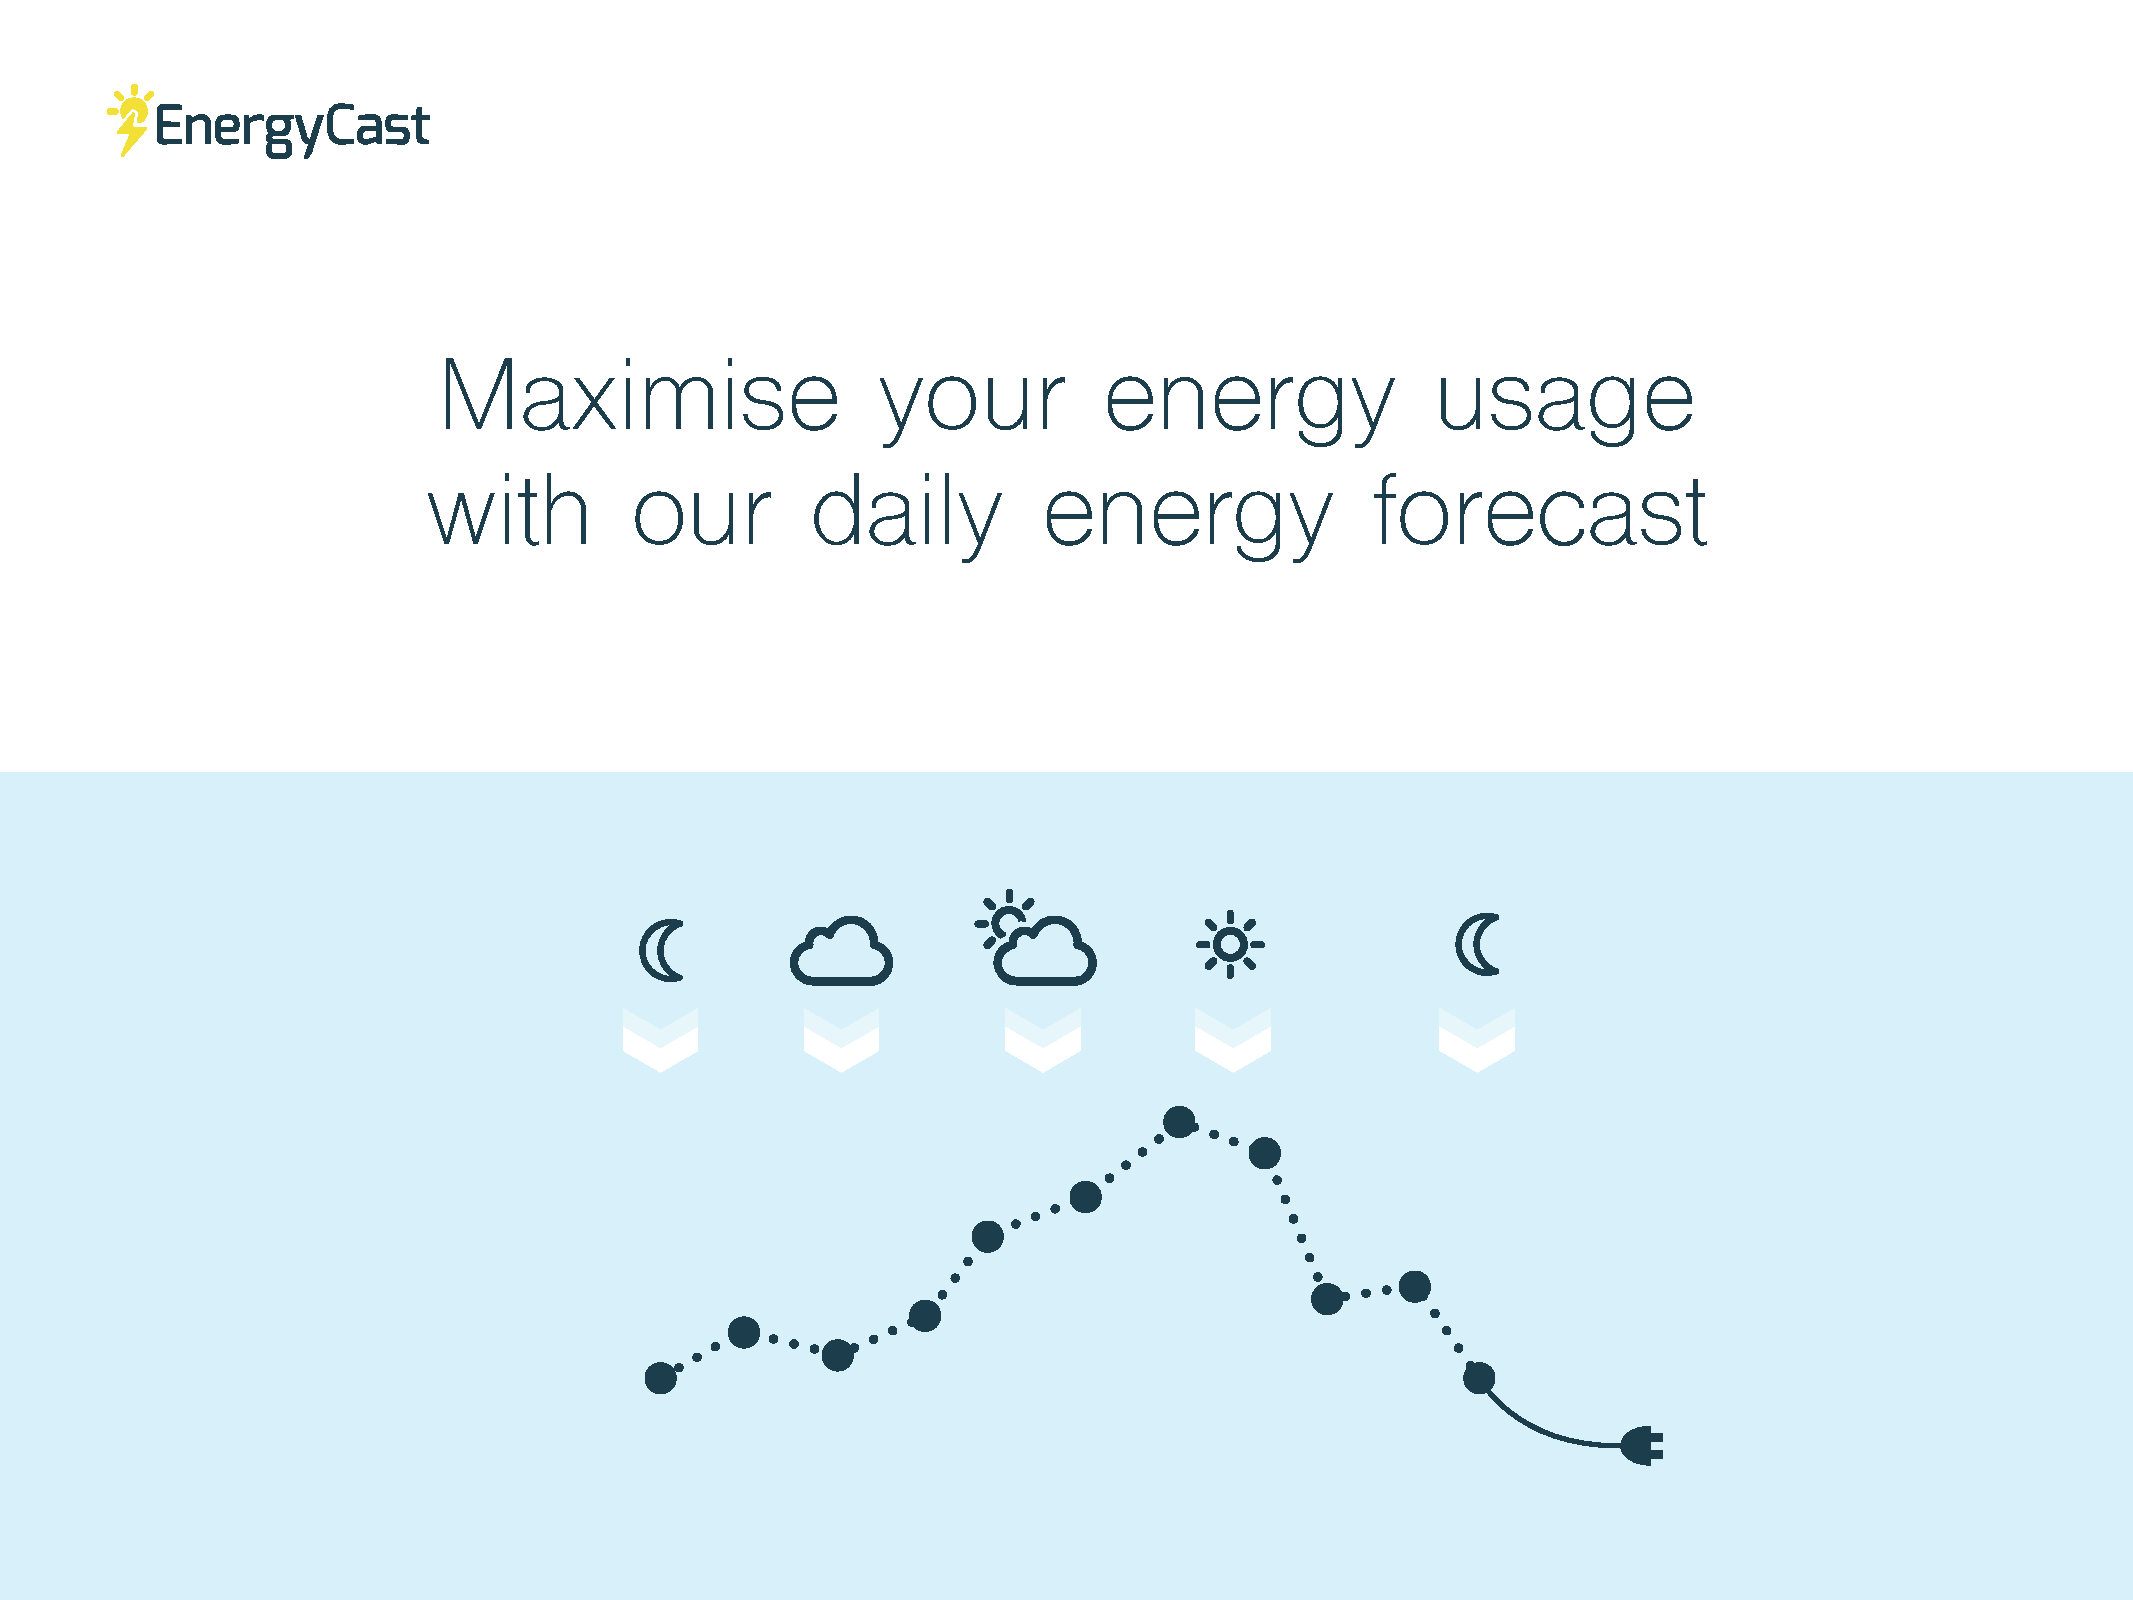
\includegraphics[height=0.8\textheight]{pic/energycast-gaphic.pdf}
		%\caption{Locust attack}
	\end{figure}	
	\end{frame}

\begin{frame}{System overview}
	
	\begin{figure} %this is tikZ figure! dont include .tex
		%	\centering
		%	\includestandalone[height=.8\textheight]{pic/SoftwareWorkflow}
		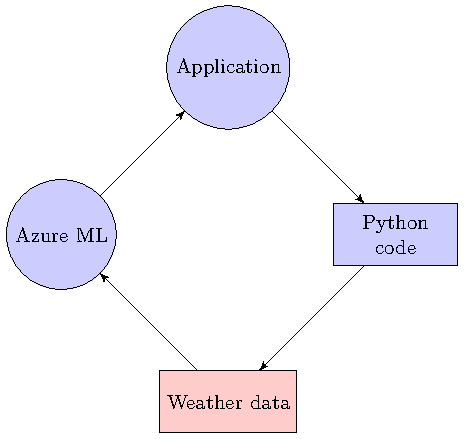
\includegraphics[width=0.7\textwidth]{pic/SoftwareWorkflow.pdf}
		
		%\caption{System overview}
	\end{figure}
	
	\url{http://envirohack.herokuapp.com/}
\end{frame}

\begin{frame}{Unlocking data}
	\begin{figure}
		\centering
		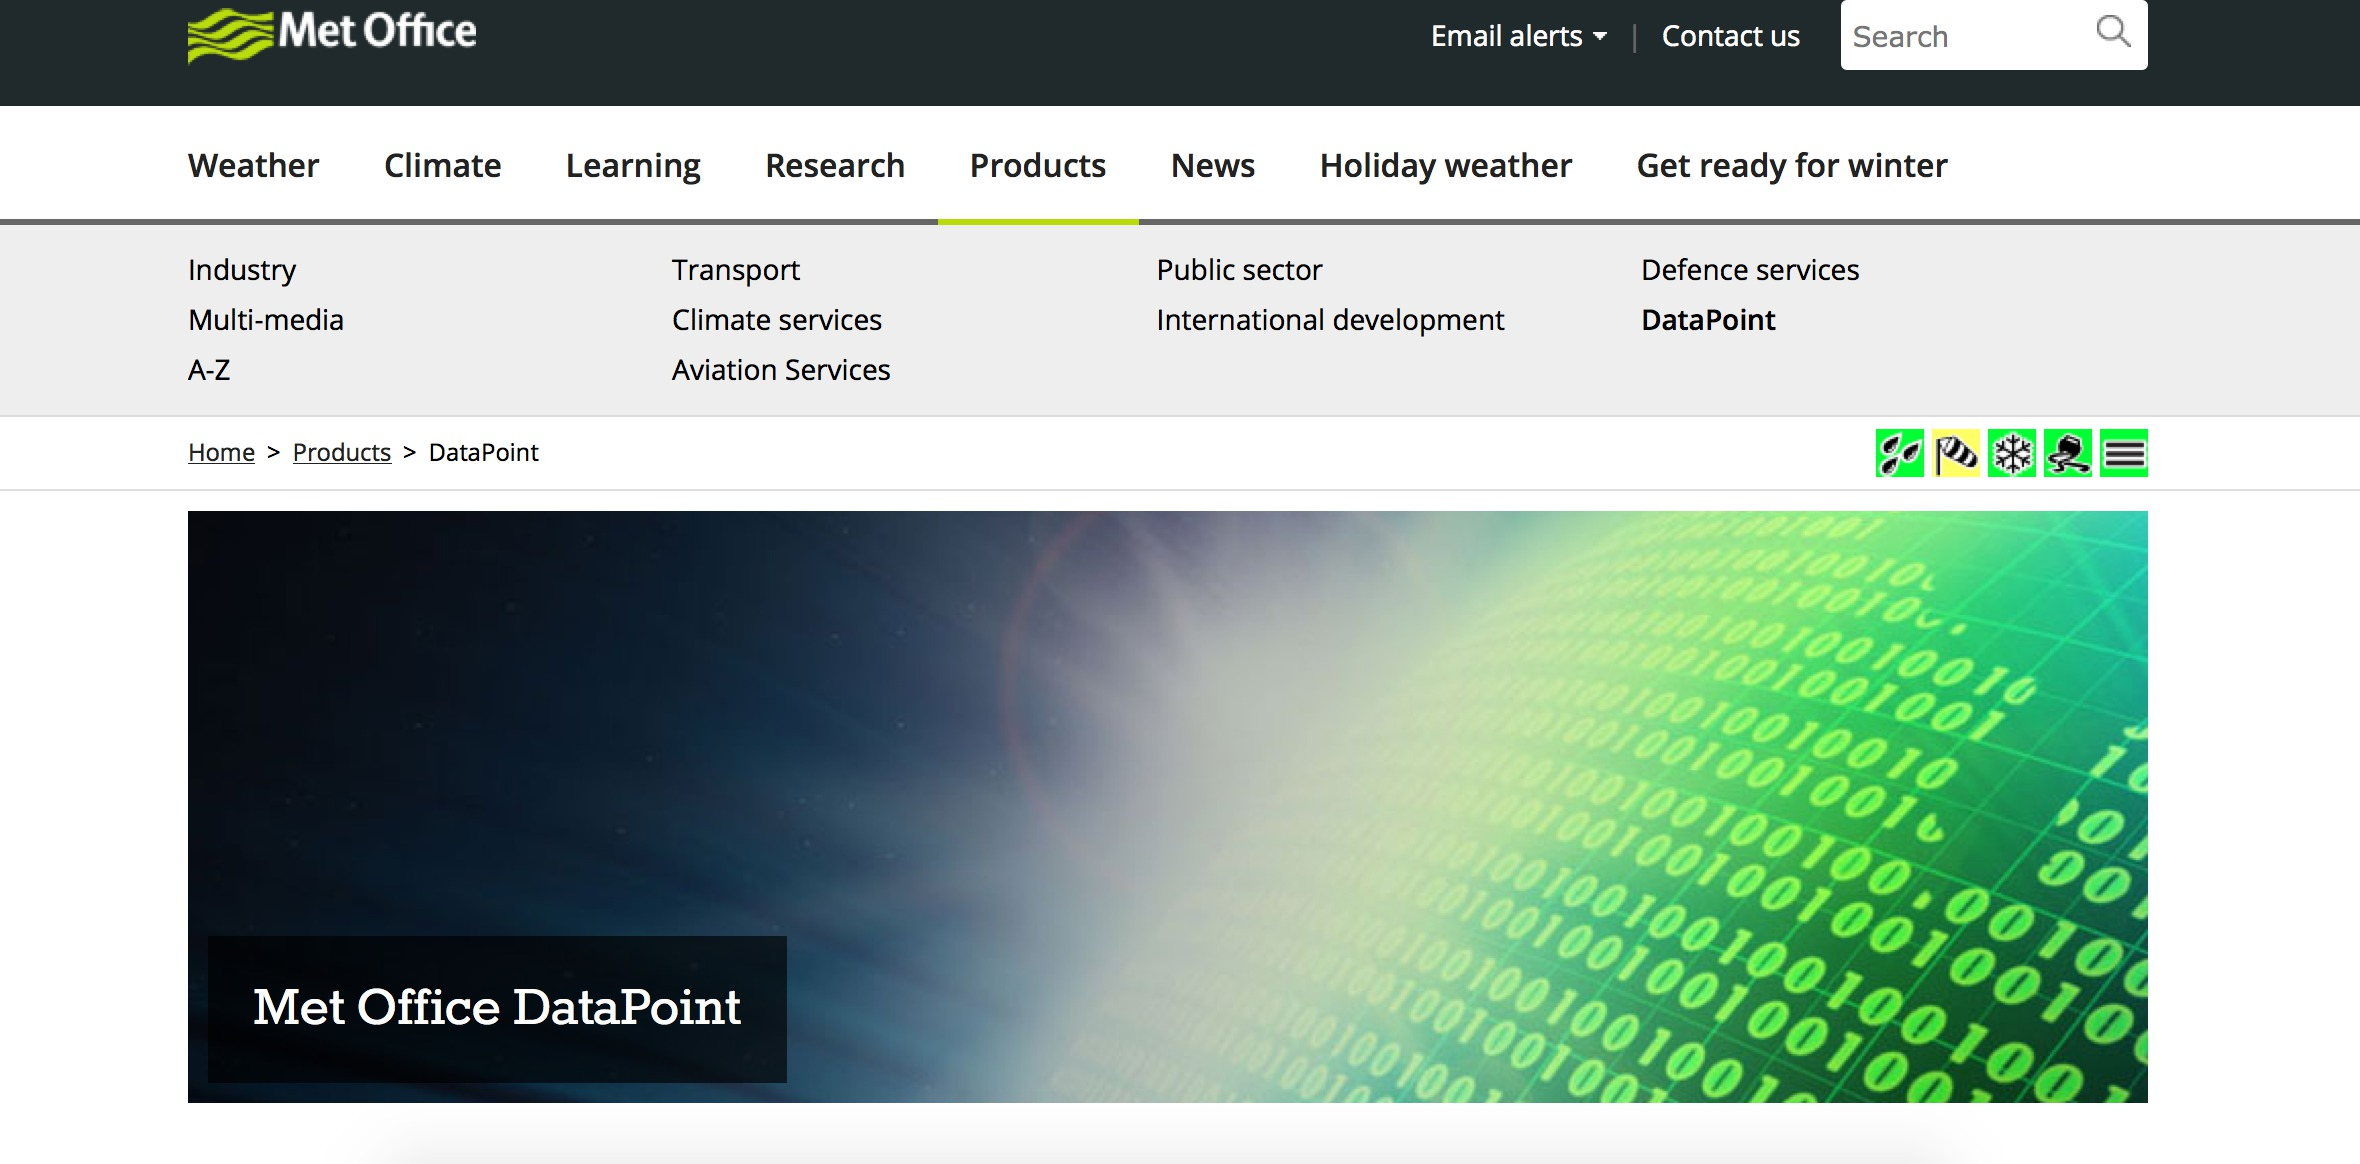
\includegraphics[width=1.0\textwidth]{pic/dataPoint.jpg}
		%\caption{Locust attack}
	\end{figure}

\end{frame}

\begin{frame}{Machine Learning}
	\begin{figure}
		\centering
		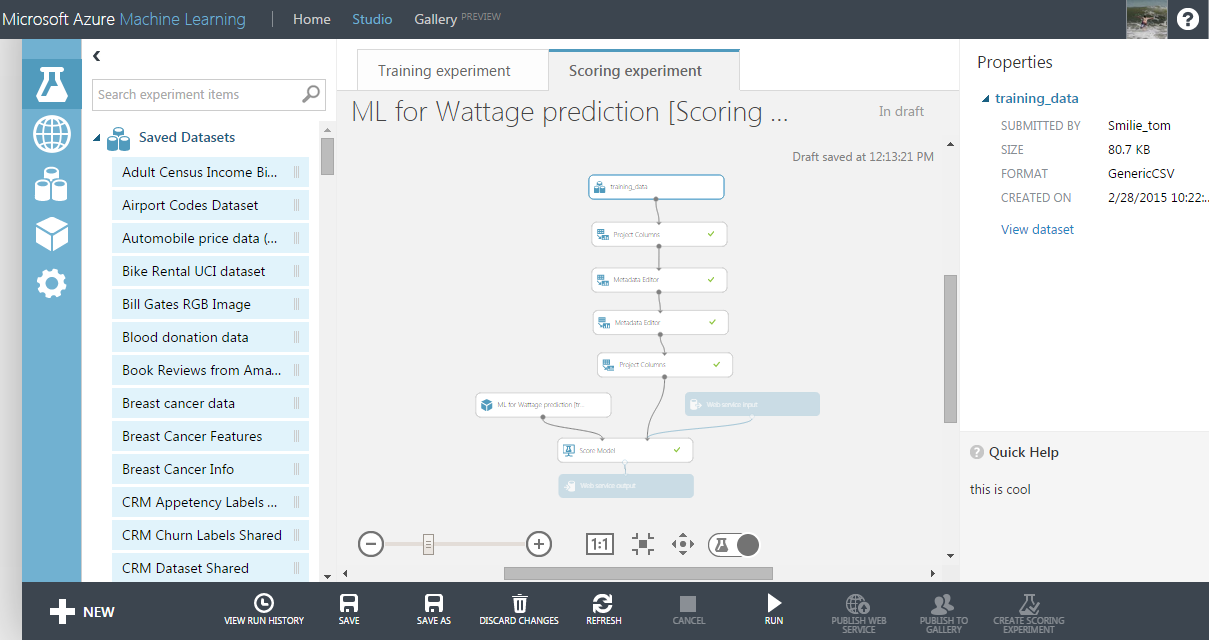
\includegraphics[width=1.0\textwidth]{pic/MLmodel.png}
		%\caption{Locust attack}
	\end{figure}
	
	\url{http://envirohack.herokuapp.com/}
\end{frame}

\begin{frame}{Machine Learning model accuracy}
	\begin{figure}
		%\centering
		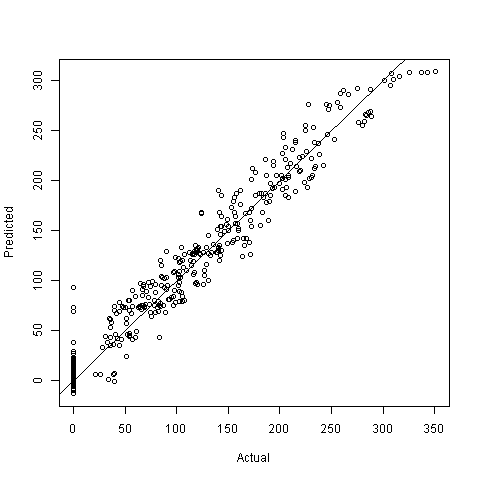
\includegraphics[height=0.9\textheight]{pic/MLaccuracy.png}
		%\caption{Locust attack}
	\end{figure}

\end{frame}


\begin{frame}{Taking things forward}
\begin{Large} %make text large
	\begin{itemize}
		\item Smart information
		\item  Smart decisions
		\item Smart devices
	\end{itemize}
\end{Large}
\end{frame}

\end{document}
